\chapter{\lr{MLOps}}\label{ch:HVS}
 
\section{مقدمه}
 
در حالی که مدل‌های یادگیری ماشین به طور گسترده‌ توسعه یافته‌اند، انتقال آن‌ها از مفهوم آزمایشی به محیط تولید اغلب با شکست مواجه می شود. این فاصله بیشتر به خاطر این است که تاکنون توجه اصلی روی ساخت مدل‌ها بوده است، نه روی تولید محصولات یادگیری ماشین که قابلیت استفاده در محیط تولید را دارند. علاوه بر آن، مدیریت بخش‌ها و زیرساخت‌های پیچیده‌ای که برای یک استقرار موثر ضروری هستند نیز در این امر مغفول مانده اند. برای رفع این مسئله، مفهوم عملیات یادگیری ماشین یا \lr{MLOps} معرفی شده است. \lr{MLOps} بر روی خودکارسازی و عملیاتی کردن فرآیندهای یادگیری ماشین تمرکز دارد تا انتقال پروژه‌های یادگیری ماشین از مفهوم به تولید را تسهیل کند. این رویکرد شامل دیدگاه جامعی از طراحی سیستم، هماهنگی اجزا، تعریف نقش‌ها و مسئولیت‌ها می باشد. هدف کاهش خطا به منظور افزایش قابلیت اطمینان و کارایی سیستم‌های یادگیری ماشین در کاربردهای واقعی می باشد. این فصل به بررسی تعریف، اصول، ابزار و معماری جامعی از یک پلتفرم  \lr{MLOps} پرداخته و در نهایت، محصولات و رقبا این حوزه را بررسی می کنیم.

\section{تعریف مفاهیم اولیه}

\lr{MLOps}
 یا عملیات یادگیری ماشین به مجموعه‌ای از فرایندها، ابزارها و شیوه‌ها جهت مدیریت چرخه توسعه مدل‌های یادگیری ماشین در یک محیط عملیاتی اشاره دارد. همچنین این چرخه شامل همکاری بین دانشمندان داده و مهندسان \lr{DevOps} است به گونه ای که این اطمینان حاصل شود که مدل‌ها به طور مؤثر توسعه، استقرار، پایش و به‌روزرسانی می‌شوند. هدف \lr{MLOps} افزایش سرعت، قابلیت اطمینان و مقیاس پذیری مدل‌های یادگیری ماشین و فرایند توسعه این مدل ها در تولید است؛ درحالی‌که خطرات ناشی از ریسک عدم موفقیت را نیز کاهش می‌دهد. همچنین به‌کارگیری \lr{MLOps} فرایند مدیریت را ساده‌تر کرده، کیفیت را افزایش می‌دهد و استقرار مدل‌های یادگیری عمیق و یادگیری ماشین در محیط‌های تولید با مقیاس بزرگ را خودکار می‌کند. لذا می توان گفت یکی از اهداف \lr{MLOps}، بهبود خودکارسازی و ارتقای کیفیت مدل‌های تولید و درعین‌حال توجه به الزامات تجاری و نظارتی است. 
 
 
 استقرار مدل‌های یادگیری ماشین روی محیط عملیاتی در \lr{MLOps} اهمیت زیادی دارد، زیرا به سازمان‌ها کمک می‌کند تا مطمئن شوند که مدل‌هایشان در طول زمان دقیق، قابل‌اعتماد و کارآمد هستند. به‌طورکلی، \lr{MLOps} با خودکار کردن بسیاری از مراحل مربوط به استقرار و مدیریت مدل‌های یادگیری ماشین، به دانشمندان و مهندسان داده اجازه می‌دهد تا با همکاری یکدیگر به ارائه سریع‌تر و کارآمدتر مدل‌های یادگیری ماشین دست یابند. 
\subsection{اصول}
برای تسهیل در رسیدن به اهداف فوق، تیم‌های \lr{MLOps} از اصول زیر استفاده می کنند:
\begin{enumerate}
	\item 
	خط لوله خودکار \lr{CI/CD} و هماهنگ سازی جریان کار\footnote{\lr{Workflow}}:
	خودکارسازی \lr{CI/CD} شامل مراحل ساخت، آزمایش، تحویل و استقرار است که به توسعه‌دهندگان نسبت به موفقیت یا شکست مراحل مختلف بازخورد سریعی را ارائه داده و بهره‌وری کلی را افزایش می‌دهد \cite{MLOpsPipeline1}. در همین حال، هماهنگ سازی جریان کاری وظایف یک خط لوله‌ یادگیری ماشین را با استفاده از گراف‌های بدون‌حلقه‌ی جهت‌دار\footnote{\lr{Directed Acyclic Graph (DAG)}} هماهنگ می‌کند، که ترتیب اجرای وظایف را با توجه به روابط و وابستگی‌ها تعیین می‌کند. ترکیب این دو رویکرد می ‌تواند به بهبود عملکرد و کارایی تیم‌های توسعه و داده‌کاوی کمک کند \cite{MLOpsWO1, MLOpsWO2}.
	\item 
	کنترل نسخه مدل‌های یادگیری ماشین، مجموعه‌داده‌ها و کد منبع:
با استفاده از نسخه‌بندی مدل، داده و کدمنبع، می‌توان هر تغییر و اصلاحی را در طول زمان دنبال کرد، که این امر به توسعه‌دهندگان و محققان اجازه می‌دهد تا به راحتی به نسخه‌های قبلی بازگردند و نتایج را بازبینی کنند. این قابلیت برای حفظ یکپارچگی و شفافیت در پروژه‌های نرم‌افزاری و علمی بسیار حیاتی است \cite{MLOpsPipeline1}.
	\item 
	نظارت و آموزش مدوام مدل یادگیری ماشین:
آموزش مداوم\footnote{\lr{Continuous Training (CT)}} در یادگیری ماشین به معنای آموزش دوره‌ای مدل‌های یادگیری ماشین بر اساس داده‌های جدید است. این فرآیند همیشه شامل یک مرحله ارزیابی برای سنجش تغییرات کیفیت مدل است \cite{MLOpsCT1}. نظارت مداوم به معنای ارزیابی دوره‌ای داده‌ها، مدل‌ها (مانند دقت پیش‌بینی)، کد منبع و  منابع زیرساختی است تا خطاها یا تغییرات احتمالی که بر کیفیت محصول تاثیر می‌گذارند، شناسایی شوند. این فرآیند به توسعه‌دهندگان امکان می‌دهد تا به سرعت مشکلات را شناسایی و برطرف کنند و از افت عملکرد مدل جلوگیری کنند. یکی از دلایل لزوم آموزش مداوم، رانش داده یا مدل\footnote{\lr{Data or Model Drift}} است، که به تغییرات تدریجی در داده‌ها یا عملکرد مدل در طول زمان اشاره دارد و می‌تواند باعث کاهش دقت پیش ‌بینی‌ها شود \cite{MLOpsProd1}. این اصل در \lr{MLOps} برای اطمینان از عملکرد بهینه مدل‌ها و واکنش سریع به تغییرات محیطی و داده‌ها ضروری است. این فرآیند بهره‌وری را افزایش می‌دهد و کیفیت کلی سیستم‌های یادگیری ماشین را بهبود می‌بخشد. در نهایت، ترکیب آموزش و نظارت مداوم به توسعه‌دهندگان کمک می‌کند تا مدل‌ها را به‌روز نگه داشته و از تاثیرات منفی رانش داده یا مدل جلوگیری کنند \cite{MLOpsCT2}.
	
	\item 
	 ثبت فراداده\footnote{\lr{Metadata}} یادگیری ماشین:
ثبت فراداده برای هر مرحله در جریان ‌کار یادگیری ماشین شامل ثبت جزئیات هر دوره آموزش مدل، مانند تاریخ و زمان آموزش، مدت زمان، پارامترهای استفاده شده و معیارهای عملکرد مدل می باشد \cite{MLOpsWO2}. علاوه بر این، جزئیات مدل که شامل داده‌ها و کدهای استفاده شده است، باید ثبت شود تا قابلیت پیگیری کامل آزمایشات فراهم گردد. این امر به توسعه‌دهندگان کمک می‌کند تا تغییرات و نتایج را به دقت مستند کرده و در صورت نیاز به نسخه‌های قبلی بازگردند \cite{MLOpsProd2}.
	\item 
	حلقه های بازخورد\footnote{\lr{feedback loops}}:
حلقه‌های بازخورد به توسعه‌دهندگان اجازه می‌دهند تا به‌طور مداوم مدل‌ها را بهبود بخشند، مشکلات را شناسایی و رفع کنند و از افت کیفیت جلوگیری کنند. این رویکرد به تضمین کیفیت و کارایی مدل‌های یادگیری ماشین کمک می‌کند و فرآیند توسعه را به یک چرخه تکراری و قابل بهبود تبدیل می‌کند که به سرعت به تغییرات و نیازهای جدید پاسخ می‌دهد \cite{MLOpsProd2}. به عنوان مثال، یک حلقه بازخورد از مرحله مهندسی مدل آزمایشی به مرحله قبلی مهندسی ویژگی می‌تواند بسیار مفید باشد.
\end{enumerate}

می توان اضافه کرد که یکی از اصول مهم که کمتر جنبه فنی دارد و در روح فرهنگی \lr{DevOps} نیز جایگاه ویژه‌ای دارد، اصل همکاری\footnote{\lr{Collaboration}} است. این اصل بر امکان همکاری مشترک افراد بر روی داده‌ها، مدل‌ها و کدها تاکید دارد. علاوه بر جنبه‌های فنی، اصل همکاری به ایجاد فرهنگ کاری مشارکتی توجه دارد که هدف آن کاهش ایزوله سازی ‌های حوزه‌ای بین نقش‌های مختلف است. چنین رویکردی باعث می‌شود تا افراد با تخصص‌های گوناگون به طور هم‌افزا با یکدیگر کار کنند، دانش خود را به اشتراک بگذارند و از هم بیاموزند. 

\subsection{اجزاء}

پس از شناسایی اصولی که در قسمت قبل صحبت کردیم، اکنون اجزای دقیق یک معماری \lr{MLOps} را توضیح داده و ارتباط هرکدام با اصول گفته شده را بیان می کنیم. ارجاعات داخل پرانتز به اصولی اشاره دارد که اجزای فنی در حال پیاده سازی هستند. ؟؟؟؟؟؟؟؟؟؟؟؟؟؟؟؟؟؟؟؟؟؟؟؟؟؟؟؟؟؟؟؟؟؟؟؟؟؟؟؟؟؟؟

\subsubsection{سازآرایی جریان کاری}
سازآرایی جریان‌کاری\footnote{\lr{Workflow Orchestration}} به عنوان یکی از اجزای حیاتی در مدیریت و خودکارسازی جریان‌های کاری پیچیده در حوزه‌های مختلف از جمله یادگیری ماشین و مهندسی داده، نقش مهمی ایفا می‌کنند. این سیستم‌ها مانند شکل 
~\ref{fig: airflow pipelines}
از گراف‌های بدون حلقه جهت دار برای نمایش ترتیب اجرای وظایف استفاده می کنند. هر مرحله از این جریان‌کاری ممکن است شامل استخراج داده، آموزش مدل یا استنتاج باشد. این سیستم‌ها نه تنها ترتیب اجرای وظایف را مدیریت می‌کنند، بلکه وابستگی‌های متقابل بین وظایف را نیز مورد توجه قرار می‌دهند. هم چنین این ابزارها به کاربران امکان می‌دهند تا جریان های کاری را به صورت خودکار و مقیاس ‌پذیر اجرا کنند. این امر به ویژه در محیط‌های بزرگ با داده های کلان اهمیت دارد \cite{MLOpsWO2}.

ابزارهای متن باز معروف در زمینه یادگیری ماشین \lr{Apache Airflow}\cite{Airflow} و \lr{Kubeflow pipeline} می باشند. از \lr{Apache Airlfow} بیشتر برای استخراج، تبدیل و بارگذاری\footnote{\lr{Extract, Transform, Load (ETL)}}داده های بزرگ استفاده می کنند. \lr{Kubeflow Pipelines} نیز بخشی از پلتفرم \lr{Kubeflow}\cite{Kubeflow} است که برای اجرای جریان‌های کاری یادگیری ماشین بر روی کوبرنتیز طراحی شده است \cite{MLOpsWFCOMP1}. از این ابزار به طور خاص برای توسعه و استقرار مدل‌های یادگیری ماشین در محیط‌های ابری مناسب است که در فصل های بعدی با آن بیشتر آشنا خواهیم شد.	

\begin{figure}[t]
	\centering
	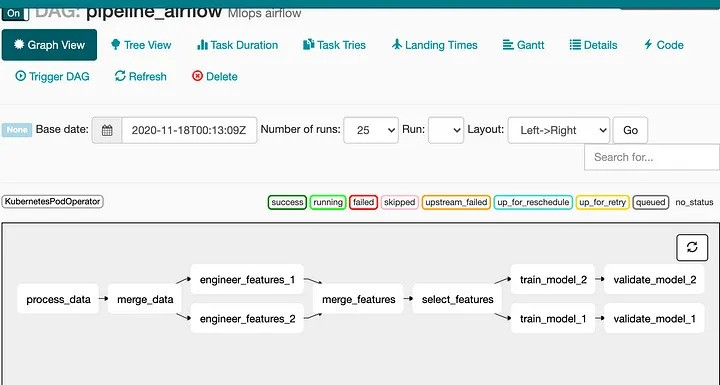
\includegraphics[scale=0.6]{Aairflow-pipeline.jpg}
	\caption{خط لوله در \lr{Apache Airlfow}}
	\label{fig: airflow pipelines}
\end{figure}

\subsubsection{انباره ویژگی}
انباره ویژگی\footnote{\lr{Feature Store}} یک سیستم مدیریت داده است که به منظور ذخیره‌سازی، مدیریت و اشتراک‌گذاری ویژگی‌های مورد استفاده در مدل‌های یادگیری ماشین طراحی شده است. این سیستم (شکل 
~\ref{fig: feature store})
دارای دو بخش اصلی است: پایگاه داده آنلاین و پایگاه داده آفلاین. هر یک از این پایگاه‌های داده نقش خاصی در فرآیند مدیریت و استفاده از ویژگی‌ها ایفا می‌کنند.

\textbf{پایگاه داده آفلاین}
برای ذخیره ‌سازی و مدیریت ویژگی‌هایی استفاده می‌شود که در فرآیندهای آزمایش و تحلیل به کار می‌روند. این پایگاه داده معمولاً با تاخیر نسبتا بیشتری نسبت به پایگاه داده آنلاین استفاده می شود و برای مواردی مناسب است که نیاز به پردازش حجم زیادی از داده‌ها در مدت زمان طولانی ‌تر دارند. ویژگی ‌هایی که در این پایگاه داده ذخیره می‌شوند، اغلب در فرآیندهای آموزش مدل‌های یادگیری ماشین مورد استفاده قرار می‌گیرند.

\textbf{پایگاه داده آنلاین}
برای ارائه ویژگی‌ها به صورت بلادرنگ استفاده می‌شود و تأخیر کمی دارد. این پایگاه داده‌ها برای سیستم‌هایی مناسب هستند که نیاز به پاسخگویی سریع دارند. زمانی که یک مدل یادگیری ماشین نیاز به استفاده از ویژگی‌ها برای انجام پیش‌بینی‌های فوری دارد، داده‌ها از این پایگاه داده آنلاین بازیابی می‌شوند. این نوع پایگاه داده‌ها باید توانایی پشتیبانی از بارهای کاری سنگین و حجم بالای درخواست‌ها را داشته باشند تا بتوانند عملکرد مطلوبی را در شرایط عملیاتی فراهم کنند. ویژگی‌هایی که در این پایگاه داده ذخیره می‌شوند، اغلب در فرآیندهای استنتاج مدل‌های یادگیری ماشین مورد استفاده قرار می‌گیرند.


با استفاده از انباره ویژگی توسعه‌دهندگان می‌توانند ویژگی‌های از پیش پردازش شده را به صورت متمرکز ذخیره کرده و به راحتی در پروژه‌های مختلف به اشتراک بگذارند، که این امر به تسریع فرآیند توسعه مدل‌ها و بهبود دقت پیش بینی ها کمک می‌کند. این سیستم‌ها معمولاً بر روی زیرساخت‌های ابری اجرا می‌شوند تا مقیاس‌پذیری بالا و کارایی مورد نیاز برای پردازش داده های کلان را فراهم کنند \cite{MLOpsCT2}. از ابزار معروف متن باز برای می توان به \lr{Feast}\cite{Feast} اشاره نمود.

\begin{figure}[t]
	\centering
	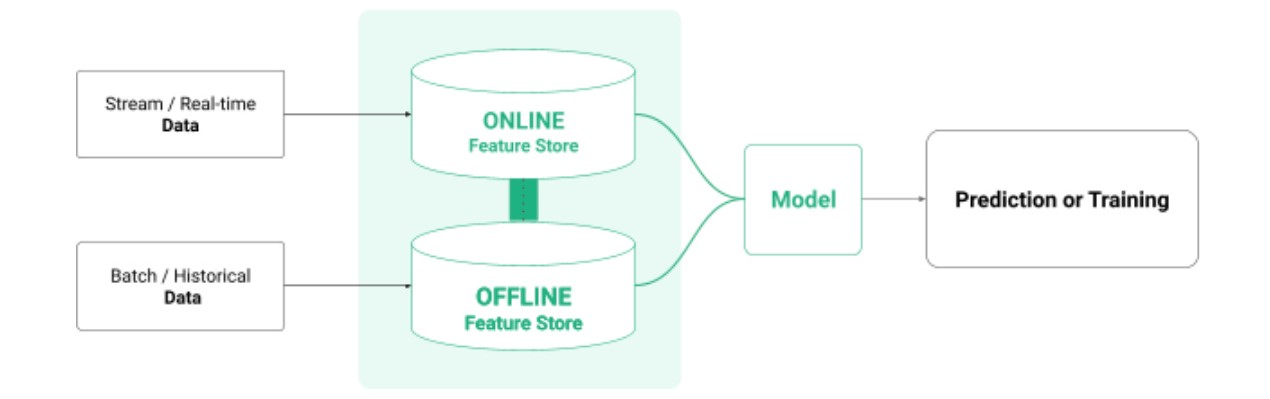
\includegraphics[scale=0.3]{feature-store2.jpg}
	\caption{انباره ویژگی}
	\label{fig: feature store}
\end{figure}

\subsubsection{مخزن کد منبع}
مخزن کد منبع به عنوان یک نقطه مشترک برای نگهداری و مدیریت کدهای مربوط به مدل‌های یادگیری ماشین یک سازمان عمل می‌کند. با استفاده از سیستم‌های مدیریت نسخه مانند گیت، تیم‌ها می‌توانند به راحتی تغییرات کد را پیگیری کرده و در صورت لزوم به نسخه‌های قبلی کد بازگردند. این مخزن همچنین به خودکارسازی فرآیند \lr{CI/CD} کمک می‌کند، به طوری که هرگونه تغییر در کد به طور خودکار خط لوله را فعال کرده و  تغییرات تست، ارزیابی و در محیط‌های مختلف مستقر می‌شوند. می توان از ابزار متن باز برای پیاده سازی آن به \lr{GitLab}\cite{GitLab} و \lr{Gerrit}\cite{Gerrit} اشاره نمود.
\subsubsection{خط لوله \lr{CI/CD}}
همان طور که در گذشته نیز راجع به آن صحبت کردیم، خط لوله \lr{CI/CD} به تیم‌ها اجازه می‌دهند تا کدهای مدل و داده‌ها را به‌صورت مداوم تست، تأیید و استقرار دهند. در این فرآیند، مدل‌ها به طور خودکار بازآموزی و بهبود می‌یابند و در محیط‌های مختلف (توسعه، تست، تولید) به صورت پیوسته به‌روزرسانی می‌شوند. این کار نه تنها باعث افزایش کیفیت و دقت مدل‌ها می‌شود بلکه زمان توسعه و عرضه را نیز به طرز قابل‌توجهی کاهش می‌دهد. در \lr{MLOps} این خط لوله ‌ها در مراحل مختلف از جمله آموزش مدل، ارزیابی، استقرار و نظارت بر عملکرد مدل‌ها و هم چنین داده ها استفاده می‌شوند \cite{MLOpsProd2}. از ابزارهای مناسب برای این کار می توان به \lr{Jenkins}\cite{Jenkins} و \lr{GitLab CI}\cite{GitLab} نام برد. 



































